% !TEX root=nonusecomments.tex
\section{Findings}
\label{sec:findings}

To answer \textit{RQ1} and \textit{RQ2} we present the findings of sentiment coding and thematic coding respectively here:
\subsection{RQ1: Sentiment Coding}


Table~\ref{tab:table1} and Table~\ref{tab:table2} summarizes the categories assigned by the raters after coding all 2000 comments from Slashdot and 1000 comments from Schneier's blog respectively. Only 134 (6.7\%) times for Slashdot and 23 (2.3\%) times for Schneier's blog the raters disagreed. Since we got a high agreement score, we picked 1022 (888+109+25) and 320 (297+12+11) comments respectively which were marked as \textit{NS} by one or both the raters for second level thematic coding.



\newcommand{\head}[1]{\textnormal{\textbf{#1}}}



\begin{table}[!ht]
% let LaTeX figure out optimal amount of intercolumn whitespace:
\setlength\tabcolsep{0pt} 

\begin{tabular*}{\columnwidth}{@{\extracolsep{\fill}}c*{3}{T{1.8}}cT{1.8}}  
\toprule
\head{First/Second Rater} & \head{NS} & \head{NRNS}\\
\midrule
\textbf{NS}              & 888     & 109 \\                    
   \textbf{NRNS} & 25      & 972     \\
  \hline
\bottomrule 
\end{tabular*}
\caption{Categories assigned by two independent raters on 2000 Slashdot comments. (NS = Negative Sentiment, NRNS = Not Related to Negative Sentiment)}
    \label{tab:table1}
\end{table}



\begin{table}[!ht]
% let LaTeX figure out optimal amount of intercolumn whitespace:
\setlength\tabcolsep{0pt} 

\begin{tabular*}{\columnwidth}{@{\extracolsep{\fill}}c*{3}{T{1.8}}cT{1.8}}  
\toprule
\head{First/Second Rater} & \head{NS} & \head{NRNS}\\
\midrule
\textbf{NS}              & 297     & 12 \\                    
   \textbf{NRNS} & 11      & 680     \\
  \hline
\bottomrule 
\end{tabular*}
\caption{Categories assigned by two independent raters on 1000 Schneier's blog comments. (NS = Negative Sentiment, NRNS = Not Related to Negative Sentiment)}
    \label{tab:table2}
\end{table}






\subsection{RQ2: Thematic Coding}
 Later, we performed second level thematic coding based on 10 themes mentioned previously to see what is the underlying factor for either social media \textit{Non-use} or user dissatisfaction. The findings are summarized in Table~\ref{table:coding category} (see the overall columns). We have shown, for each theme, the number of \emph{NS} comments that fell into that theme. The percentages shown in parentheses does not sum to 100 since one comment could be associated with multiple themes therefore those comments are counted multiple times (also percentages are calculated for individual dataset and not as a whole). We explain the themes with example comments in detail here. For the purpose of comparison we report the findings of two data-set separately under each theme:
 
\begin{table*}[t!]
\centering
\begin{tabular}{|c|c|c|c|c|}
\hline

\multirow{2}{*}{\head{Theme}} & \multicolumn{2}{c|}{\head{\#Comments (Slashdot)}} & \multicolumn{2}{c|}{\head{\#Comments (Schneier's Blog)}} \\
%\head{Theme} & \head{\#Comments (Slashdot)} & \head{\#Comments (Schneier's Blog)}  \\
\cline{2-5} 

 & Overall & \emph{Explicit Non-use} only & Overall & \emph{Explicit Non-use} only \\

\hline
Politics/Political content     &  30 (2.93\%) & 5 (0.01\%) & 1 (0.31\%) & 0 (0\%) \\\hline

Privacy and security concerns  &  432 (42.27\%)& 138 (44.37\%) & 212 (66.25\%) & 111 (68.94\%)\\\hline

Uninteresting/unverified content  & 39 (3.81\%)& 8 (2.57\%) & 28 (8.75\%) & 12 (7.45\%)\\\hline

Fake accounts/Bots  & 5 (0.49\%)& 2 (0.64\%) & 22 (6.87\%) & 8 (4.96\%)\\\hline

User experience   & 341 (33.36\%)& 118 (37.94\%) & 41 (12.81\%) & 18 (11.18\%)\\\hline

Switch to other sites/services  & 18 (1.76\%)& 8 (2.57\%) & 18 (5.62\%) & 10 (6.21\%)\\\hline



Psychological impact   & 9 (0.88\%)& 1 (0.32\%) & 7 (2.18\%) & 3 (1.86\%)\\\hline

Advertisement   & 104 (10.17\%)& 21 (6.75\%) & 14 (4.37\%) & 5 (3.1\%)\\\hline

Personal preference  & 147 (14.38\%)& 42 (13.5\%) & 94 (29.37\%) & 68 (21.86\%)\\\hline

Other   & 35 (3.42\%)& 11 (3.53\%) & 34 (10.62\%) & 14 (8.69\%)\\\hline
\hline
\end{tabular}
\caption{Themes from second level thematic coding and number of comments for both dataset (separately we show for overall \emph{NS} comments, \emph{Explicit Non-use} only comments)}
    \label{table:coding category}
\end{table*}
 
 \subsubsection{Politics/Political content}
 Slashdot users often mention about posts talking specifically on the social or the political contexts which they think is not appropriate for Facebook: ``\textit{I quickly learned to use the ``mute'' feature in Facebook because of those idiots who post zero impact political comments. You know, those comments that won't convince the other side and that people who already agree with the position don't need to read, yet idiots keep posting that and no doubt high-five themselves as they re-read their masterpiece.}'' Here the user is clearly frustrated with the way people post political content. It should be noted that this commenter expressed how his interaction with Facebook has changed due to the audience activity. Some of the users questioned the credibility of the news sources in Facebook: ``\textit{Facebook does have credibility?
Was that before or after Facebook admitted to promoting pro-Hillary and suppressing pro-Trump stories/outlets?}''
    
Some of the users explicitly indicated political contents are why they prefer to endorse \emph{Non-use}: \textit{``And this is why you don't go on Facebook ever. Well that, and I literally couldn't give less of a damn about the kind of leftist drivel that populates most of any social media.''} Meanwhile others blamed Facebook to keep them in `political bubble', such as: ``\textit{Yes, Facebook is keeping me in a political bubble, but not nearly to the extent that National Review did in the early 90s...}''
    
One commenter of Schneier's blog indicated his apprehension that Facebook CEO Mark Zuckerberg is capitalizing the big data to create his own intelligence service and he calls it some kind of `oligarch plum'. Some criticized Facebook by claiming it is the worldwide censor of those who manipulate civic discourse: ``\textit{...On top of that, Mr. Zuckerberg is reportedly preparing for a presidential run. The appearance is with his big money and data access he is trying to buy the presidency... I must ask, what is positive discourse and who decides which is which and by what criteria? Can Facebook and it's executives be trusted? }''

 \subsubsection{Privacy and security concerns }
 Privacy and security has been a major concern for majority of the Slashdot user under study. They are particularly disgusted by the fact that Facebook is constantly doing data mining, selling their data etc. One commenter mentioned,
     ``\textit{All this tells me is that Facebook is actively developing new, innovative ways to invade your privacy, and this particular bit of data mining technology has become reliable enough that they felt it would be good PR to create a feel-good, help-the-disabled feature out of it.}''
     
     Social media usage have been shaped and reformed over the course of time due to issues related to user privacy and security~\cite{vitak2015balancing}. One major point of concern for tech-savvy user population has been identity theft. The fact that Facebook uses the information on user profile to sell it to other party make them skeptical about their future engagement with it. One such user wrote,
     ``\textit{By signing up for Facebook, you surrender your identity as it is - maybe this is to take it to the next level. They will stream everything these people do for our entertainment. That's the price they would have to pay to live there.}''
    
    However, one user argued by saying although he does not have a personal account, he might cosider having a corporate account since it is a good way of reaching people: \textit{``...Never had an account on FB...never will...I don't want to give any personal info to them, but I would consider a business only account if they offered one.''} One recurrent quote that emerged from these category comments was: \textit{``...Got sick of the privacy issues, having my personal information being sold for money (while I get NO benefit from it)...''} Another set of users do not like the Facebook terms of service for having to use the original name to create the account: ``\textit{Not to mention, Facebook's TOS is that you must use your real name when creating an account. If FB cared one whit about privacy it would let people uses aliases. It really is incredible how ghetto and scammy FB is with their tactics and policies.}'' 
    
    Slashdotters are also apprehensive of the lack of security of Facebook source code and some of them wanted it to be open source: \textit{``Security. If Facebook source code was open, security flaws which are disclosed every one day or another, probably ruining life of thousands due to privacy leaks, would have been closed faster...''}. Privacy violation and security breach is one major point of concern of many users who think Facebook do not consider this seriously enough: ``\textit{...Of course, Facebook isn't the only company guilty of this type of thing -- and I suspect that until there is some serious consequence associated with this type of security hole, most companies won't take it seriously enough.}''
    
    Privacy and security is the primary concern for \emph{NS} and \emph{Non-use} of Schneier's blog users as well. Not everyone is very polite about the privacy violation of Facebook: \textit{``So if G and FB are OK with privacy being dead, why don't they share the details of their advertising operations and source code? Or do they mean privacy is dead for everyone but themselves?''} The amount of surveillance (storing metadata, emails, phone call etc.) and tracking that comes with a Facebook account is worrying for common mass: \textit{``... If facebook can do it, the NSA can do it, too. In a few years, everybody can do it. This is one of the reasons why I don't have pictures of myself on facebook.''} Time and again it is argued that Facebook has monopolized the social media business and the major incentive here is money instead of better service. People offered suggestions on how to avoid being tracked: \textit{``I have a fake account of facebook, it's useful when researching. Considering I use it as an information resource and since I value my privacy, there is no way I would put my personal information on there! Muffin got it right. Don't use it.''} Another workaround proposed was to use dedicated browser: ``\textit{The simple answer is do not install the facebook App, ever. If you have to go onto facebook, then do so with a dedicated browser that you use for nothing else (except maybe LinkedIn if you have to go there) as they try to track and log wherever you go on the web. Facebook strip-mines your personal data for their monetary gain...}''

    
 \subsubsection{Uninteresting/unverified content }
 This theme appeared in multiple comments where the users expressed their detest to inappropriate, irrelevant or uninteresting content on Facebook shared by other users which do not satisfy their taste. For example: ``\textit{I see very little content that's actually from the people I follow. 99\% of what I see is just stuff reshared from other places. I hardly ever use Facebook anymore because most of that reshared content doesn't interest me anyway.}'' Facebook has been considered a source of spreading propaganda and hoax since its inception. Also users considered it to be a medium for assaulting people personally by trolling and abuses which caused both \emph{explicit Non-use} and \emph{implicit NS}:
``\textit{I still don't have a Facebook account, and am no worse the wear for it. I have noted that of my family and friends who do have accounts, the ones who typically talk about their Facebook activity the most are definitely the women, and a lot of that talk seems to swing between gossip and outright vicious assaults. I'll just stay out of that mess, thanks.}''

While some users remarked, \textit{``...Facebook these days seems to just be an outrage platform with different sides all screaming at each other and nobody listening...''}. Another user reiterated, ``\textit{People seem to use Facebook as a kind of mental chewing gum. There's always some gossip and ``news'' to scroll through. Sometimes you're interested in something of it. An endless on-the-go stream of gossip.}''

Facebook is one of the biggest source of online trolling and fake news. Fake profiles and spamming are also abundant, one user mentioned why he has \emph{NS} by the infinite trolling and fake news: ``\textit{I wouldn't be surprised if readership is falling. After I had to open a FB account last year, it looked interesting for about a week, then it became an annoyance, now it seems to be troll land...And as quickly as fake news is deleted, new ones will pop up, and will make note of being deleted, which will feed into conspiracies.}''

We read varied comments belonging to this category in Schneier on Security. It is commonly observed that Facebook users live in a world of delusion and they `survive on their own filtered image'. One commenter wrote, \textit{``...On ``opting out'' of Facebook affecting your social life, I agree with Ed...REALLY? If Facebook contact, which is hardly face to face and certainly not person to person, is your social life, then you may have no life at all...Facebook et al, reminds me of something I have observed in the schools of America today, called the ``liars club''...''} Apparently, content and audience is an influential factor for any technology adoption. People care about how the platform moderates its audience and control its content. commenters of Schneier on Security tend to be more harsh with Facebook's disregard with fake profiles and pseudonyms. One such user also thought Facebook is full of useless stuff:
``\textit{the irony I see in this is that if Facebook didn't try to imply that they care about using real names/make it so much of a ``MEATSPACE PROFILE'' (they don't, people use pseudonyms/create fake profiles lately), I wonder if Facebook would be as popular or as filled with uselessness as it tends to be.}'' Another user just thinks Facebook is a fancy place and compares it with `yearbook' by saying, \textit{``I'll be the first to admit it: I know next to nothing about MySpace or Facebook. I'm guessing you were not the type to purchase a yearbook and have all your friends scribble notes in it?...I can't help but think of these sites in those terms...''}

 \subsubsection{Fake accounts/Bots}
 Often times commenters discussed about bot accounts, fake profiles, or provoking others to have a fake account. One user was worried if such flexibility of creating multiple accounts can stimulate crime. For instance, ``\textit{Since Facebook doesn't verify your identity when signing up for an account.... how long before the bad guys start setting up fake accounts or hacking FB accounts and ransoming people?}'' Fake account and bot accounts are criticized~\cite{ferrara2016rise} by users since they can be used to purchase fake likes or post reviews for business:
    ``\textit{Because I have a hard time believing that 1/7 of the world population is actively on Facebook and I also know full well that there are millions of bot accounts whose likes are purchased.}''
    
    Users of Schneier on Security also addressed this issue. Often times they chastised Facebook for the `like business': \textit{``1,000 Facebook likes for \$29.99 The unknowable number of times FB has betrayed, bamboozled, lied to and scammed their own user base makes it quite difficult for me to have even one byte of sympathy for Mr. Z and his shaky marketing company.''} One user thought negative reputation online can be shed easily by creating a new persona and thus positive reputation are vulnerable to `Sybill attacks':
    ``\textit{...If these two problems are solved a lot of problems would immediately vanish of the net. i.e. like sellers on Facebook... fake reviews in online shops. Solving this key problem of pseudonymity in a cheap way without breaking anonymity seems hard.}''
    
    Our findings suggest that Schnier on Secuirty users are more critic compared to Slashdotters in castigating Facebook for providing myriads of misinformation and intrusion. One of them suggested, \textit{``Technologists and inventors need to work on cutting Facebook off at the knees. Disposable identities, fake searches, encrypted fake traffic, photos of non-existent people, artifical-intelligence tools for generating fake blogs and comments, fake clicks, a tsunami of false information...''}
    
 \subsubsection{User experience}
 This category specifically attributes to all the Facebook feature that users didn't like e.g., the large internet data intake, problem in surfing the site, unhappy with video features, etc. One such unhappy commenter mentioned, ``\textit{Not a fan of this idea. FB Messenger spams could exceed the data caps on mobile plans (\$\$\$) and create a backlash from angry customers.}''
    
    The ability to control the profile (e.g., customizing the privacy and security settings, enable/disable features) is an important factor for users. When that ability is inhibited, user dissatisfaction escalate, such as: \textit{``Just went into my profile to try to remove / disable this POS and you are not even given the option to do so...I am so close to closing my Facebook account it is not even funny anymore.''} Also few users complained about the lack of simplicity in the Facebook interface:
    ``\textit{I'm surprised no one mentioned the disgusting interface Facebook has. It really seems badly made and unsophisticated. There are virtues in simplicity, but Facebook's take on interface is pauperism.}'' Similar arguments were maid by another user who said, \textit{``If facebook continues to make its site user-unfriendly, I'll simply stop using facebook. I've already dropped back on my usage because I cannot view my timeline the way I want to view it...''}. Some users mentioned they just use it for the sake of keeping in touch with everyone else and scheduling events:
    ``\textit{Why are people still using Facebook? Because other people are, and they use it as their medium to schedule events and coordinate activities.}'' It is often upsetting the amount of narcissism introduced by Facebook nowadays. One user mentioned Facebook users are attention-seeking and that \textit{``An hour on facebook will make you hate humanity.''} 
    
The poor Facebook \textit{user experience} among Schneier's blog users were also prevalent. A lot of them mentioned it is annoying that Facebook gather information of people who do not even have an account: ``\textit{Scarier, is that you don't even need to have a Facebook account for them to have a dossier on you. All it takes is countless ``friends'' uploading their contact list to try to maximize friendship.}'' Another user mentioned about stupid friend suggestion made by Facebook: \textit{``The whole ``people you may know'' thing is kind of creepy. I once had Facebook suggest a person who had died not long before the friend suggestion.''} Similar \emph{NS} was found while another user described the Facebook's high false positive rates in friend matching: \textit{``...I find it quite hard to believe that Facebook matches people who happened to be in the same location for some time. That would generate an awful high number of false positives...''} 
    
 \subsubsection{Switch to other sites/services}
 Some of the users preferred other social media platforms since they found them to be more useful compared to Facebook. One user considered change of Facebook's overall audience age into older people: 
     ``\textit{For people with a large audience, there's Twitter, until Facebook buys it. But there's no way to stop an old-fashioned listserv. Does anybody make a friendly one any more?}'' A common theme for this category which was interesting is a part of expert users of Slashdot consider Facebook is mostly old-fashioned and teenagers do not use it anymore: \textit{``The kids have already moved to Snapchat. Old people will no doubt stay with Facebook forever, but that's the end of growth and growth is holy in Silly Valley...''}. Those who think Facebook is not worth their while prefer to communicate via other sources e.g., email, text etc.:
    ``\textit{ But I tell ya what -- Facetwat is not on my phone. (yes, Facetwat is my derisive mashup of Facebook and Twitter.) And no, Twitter isn't on my phone. Neither is Tinder, or Snapchat or whatnot. You wanna reach me? Email me. Text me. iMessage me. Or fucking call me.}''
    
    Similar tendency is also observed among Schneier's blog commenters. Those who think Facebook has security issues and is not trustworthy, prefer other modes of communication. For example, one such user wrote, \textit{``.. In any case, I wouldn't trust anything from Facebook as far as security/privacy goes. I use Signal.''} Another user discussed what alternative of Facebook are currently there where the user does not have to compromise his privacy:
    ``\textit{...There is already an alternative project being created. Does nobody know about Diaspora* ? It's open source and distributed, with no central company collecting all your private data....If you have privacy issues with Facebook, spread the word about Diaspora!...}''
    


 \subsubsection{Psychological impact}
  Depression causes some user to stop or reduce using social media because they either think that their life is too boring compared to their online friends or that the friends sharing their highlights are fake. One such comment was: ``\textit{The negative impact social media has on the human psyche is, in my opinion, quite significant. FOMO, self-esteem issues and F4ceb00k depression are real things and they exist with a measurable amount of people who live through mass social media. Social media emulates belonging to a community whilst at the same time causing us to drift further and further apart.}''
    
    Facebook has long been accused of creating frustration and depression among teenagers who think their friends have better social life than that of theirs. One of many such comments was: \textit{``...Quitting Facebook was one of the best decisions that I ever made. Nothing good comes from it. It encourages us to compare ourselves negatively to others whom may have more money or more success. Facebook is psychologically damaging.''} It is argued that being on a social media like Facebook can deteriorate the mental health of people who are already suffering: ``\textit{The problem with social media (not just FB) and depression is not that people do nothing but stare at FB and get depressed. The problem (or, one of them) is that if you're already depressed, viewing social media can make it worse. Why? Well, because people like to present their best side on social media...}''
    
    One user of Schneier on Security tried to explain the co-relation of mental health and social media by saying majority of the US (``a pill-popping nation'', as he says) population are suffering from anxiety disorder and depression and \textit{``...the masses are unstable and the trend is worsening - Social media correlations with higher rates of reported mental illness (ironically this study used Twitter) - Life is harder in the US with worsening economic conditions (the Great Recession never ended), stagnating wages and worsening wealth and income inequality.''} Some users also mentioned how Facebook takes toll on a Family life and create loneliness: ``\textit{...If your kids did not grow up in the age of Facebook, then it is uncharted territory to you. You dont know the dangers, the addiciton, the toll it takes on a family as they drop all activities and everything, for Facebook activity...}''
    
 \subsubsection{Advertisement}
 Advertisements are a major turn off for most of the users. This category often goes in parallel to privacy and security concerns of the users. One such disgruntled user sarcastically commented, ``\textit{Don't be silly -- when Facebook taps into your pleasure center, it won't be to notify your friend that you're horny, it will be to give you a dopamine hit every time you view an advertisement. Within a few days you'll want to do nothing else.}'' They feel that they should be reimbursed for the spamming that Facebook do: \textit{``if facebook is making \$1 off of my inconvenience, facebook should pay me at least .50c of that money...''} Many users expressed their contempt against the data mining that Facebook do to make targeted ads. While some of them actually like it, many don't: ``\textit{...Facebook probably mines the unencrypted messages to help form an ``advertising profile'' for you so they can better target ads at you when you're on Facebook.}''
    
    In general, the authors felt the most negative sentiment associated with Facebook experience of the Slashdot users come from advertisements exclusively and often times they encourage others to \emph{Non-use} too: \textit{``Maybe it's time for you to stop using Facebook altogether. Your continued use of the site IS their explicit permission that they can serve you their content - ads and all.''} However, some users, although dissatisfied, have accepted this as inevitable: \textit{``After all, Facebook users have NO CHOICE but to use Facebook and allow them to force you to watch ads. Really, you have no choice, none at all. Suck it up and get used to it.''}
    
    Somewhat similar arguments were made by Schneier's blog users who are more concerned with associated security hazards caused by Facebook's money making business by running ads. They feel Facebook has every information of a given user as long as the browser cookies are enabled and any site visited by that user has a Facebook like button. One user remarked, \textit{``...I'm sure Facebook has much, much more data on a given user (at least in 2012); they would have to in order to make the targeted ads... right?''} One user mentioned why he thinks the costs of social media outweighs the benefits and his reasons for social media \emph{Non-use}: ``\textit{Regarding social media, even though I'm spiteful of advertisements/marketers for a variety of reasons, it was an ad that really struck me and contributed to the many things that got me off of twitter/Facebook and all the other wannabe sites.}''
    
 \subsubsection{Personal preference}
 We coded the comments belonging to this category where there was not enough context to understand the real reason behind the \emph{NS}. Also, when people mentioned ``I do not care'', ``waste of time'', ``do not like using it'' or just hate/swear terms without really mentioning the actual reason, we inferred this was their personal choice. One such user indicated he/she is not in any social media but doing well: \textit{``...I did 4 years ago and I'm surviving just fine. No Twitter, no Facebook, no Instagram. Nothing.''} Most of the times this comments are shorter in length and straightforward. Some user recalled some previous platform that died and wished FB has similar fate: \textit{``The future does not look so bright for Facebook as they will probably suffer the same fate as usenet.Sounds like a positive outcome to me. The world would be better off without the cancer that is Facebook.''} As mentioned earlier, a lot of users consider Facebook as a pure waste of time which eventually becomes an addiction: \textit{``...Facebook is a waste of time simply because Facebook neuters your ability to reach people if you don't pay - but so far Twitter is pretty decent.''}
     
    Lack of contextual information for deliberate \emph{Non-use} was also observed for some Schneier's blog comments. Such as: \textit{``People should delete their Facebook account and other social media accounts.''} A common practice that was observed in our data was people mocking social media sites by using derogatory names; e.g., ``\textit{Honestly Bruce, you really don't need to follow the herd to Faceache and Twatter...Facebook, MySpace et al have been around for quite some time now. 6 years ISTR. While it probably wont last for ever, thats not really a flash in the pan* If you dont like Facebook (I dont), dont use it (I dont)...}''
    
    According to them the proliferation of such media are momentary and they will soon be replaced by some other `next big thing'. Sometimes \textit{personal preference} is accompanied by some other concern such as privacy/security: ``\textit{Protect yourself by forcing the authentication to happen over TLS. Or stop logging in to Facebook from public networks. OR, do the sensible thing and don't use Facebook at all.}'' We identified few comments where people acknowledge the flaws of Facebook system but they feel there is no other option and they continue to use it. One such case, according to an user, is when people need to communicate with a group of people in a shared setting with control over the mode of communication. According to him, \textit{``...If you have no need or desire of organizing or communicating with large groups of other people, then Facebook may seem pointless...''}
    
\subsubsection{Others}

Some other topics that do not encompass the aforementioned ones comprise this category. For instance one user wrote, ``\textit{The overwhelming majority of people use Facebook. They don't give a shit about the ideals of freedom and decentralization. And they outnumber us hugely.We can't ""win"" in an essentially democratic system wherein a tiny ""we"" is up against a massive horde of ""them.""}'' He thinks the internet does not endorse freedom of speech rather it is centralized and biased. Some people mentioned they did not like Facebook app because drains the battery too fast: ``\textit{Years ago I deleted the Facebook app due to excessive battery drain. Judging by how hard they have been trying to get me to install it since, I made the right decision. Besides the access to Contacts touched on in TFS, it is also tracking your location constantly...}''
    
Another common complain for Facebook \emph{NS} was stalking. A good amount of users are pissed off by the fact that employers nowadays requires the potential employees to have a Facebook account. This stems user dissatisfaction because a significant amount of job seekers probably did not have a Facebook account which make them ineligible for that job. For example, \textit{``I don't use Facebook. I am on LinkedIn but I never update anything. And I don't care. If an employer wants my years of experience they will take me as I am. If they are going to reject me because I don't waste time on Facebook, then I probably wouldn't last long there. Their loss.''} Another Slashdotter said, ``\textit{The reason employers want everyone to be on social media: They can use it to gather information about you that would be illegal or inappropriate to ask in a job interview.}''
     
The other interesting issue, if true, can engender further research and investigation is that Facebook is responsible for revenge porn and child prostitution. A commenter on Schneier's blog pointed out this: ``\textit{Due to the fact that facebook is nothing more than prostituting your social life in exchange for some IT service it makes sense that facebook should be rated XXX and that facebook should be prosecuted for boosting child prostitution if they do not take care that no child gets a Facbook account.}''
 
 

\paragraph{Explicit Non-use only}
As mentioned earlier, after the initial binary coding we picked 1022 and 320 comments those were marked as \emph{NS} respectively for Slashdot and Schneier's blog for further analysis. The aforementioned themes emerged from a combined analysis of these comments. Simultaneously we also marked whether these comments express \emph{explicit Non-use} or \emph{implicit NS}. If the comments directly express complete abandonment, reduced usage or passive usage (lurking) of Facebook then we marked them as \emph{explicit Non-use}, \emph{implicit NS} otherwise. It turned out that, 311 out of 1022 \emph{NS} comments of Slashdot and 161 out of 320 \emph{NS} comments of Schneier's blog was marked as \emph{explicit Non-use} by the coders. Since these comments are subset of all \emph{NS} comments, it is worth investigating which of the above described themes appear and in what frequency in these \emph{explicit Non-use} only comments. Table~\ref{table:coding category} summarizes the findings (percentages are calculated on number of \emph{explicit Non-use} only comments per dataset). 

%Wordtree visualization~\cite{schoenebeck2014giving} of \emph{explicit Non-use} for Slashdot  and Schneier's blog comments(that include the words ``quit'' or ``stop'') are shown in Figure~\ref{fig:figure1} and Figure~\ref{fig:figure2} respectively (the branches explains the reasons). 

Presumably, \textit{privacy and security concerns} is the majority theme in this subset of Facebook {NS} comments (44.37\% for Slashdot and 68.94\% for Schneier's blog). The next 2 prominent theme for \emph{explicit Non-use} only comments of Slashdot are \textit{user experience} and \textit{personal preference}, and vice versa for Schneier's blog. Since \textit{privacy and security concerns} and \textit{user experience} comprise substantial \emph{explicit Non-use} only comments, we did a closer inspection. It unveiled at a granular level the non-users are concerned with Facebook's default privacy and security settings, identity theft, selling personal data for ads, keeping track of user information even after logging out, automatic posting of recent activity, unsafe scam applications \& ads, fake profiles, keeping user data even after deactivation, and lack of control in news feed. For example, one commenter explained why he stopped using it: ``\textit{I used to use facebook since the early days...But then I deleted it...Got sick of the privacy issues, having my personal information being sold for money (while I get no benefit from it), and now this...}''

In terms of \textit{user experience}, they complained about poor user interface, unsolicited friend suggestion, tagging non-users in photos, stupid game requests, improper blocking of contents, irrelevant ads, faulty facial identity from photo tags etc. For example, one commenter wrote: ``\textit{...Similarly about half the photos tagged on Facebook as me are pictures of license plates. Guess what my hobby is. What I'm saying is that Facebook's idea of facial identity from photograph tags is not without problems.}''



%%%commented out region starts here%%%

\begin{comment}



\begin{figure*}
  \centering
  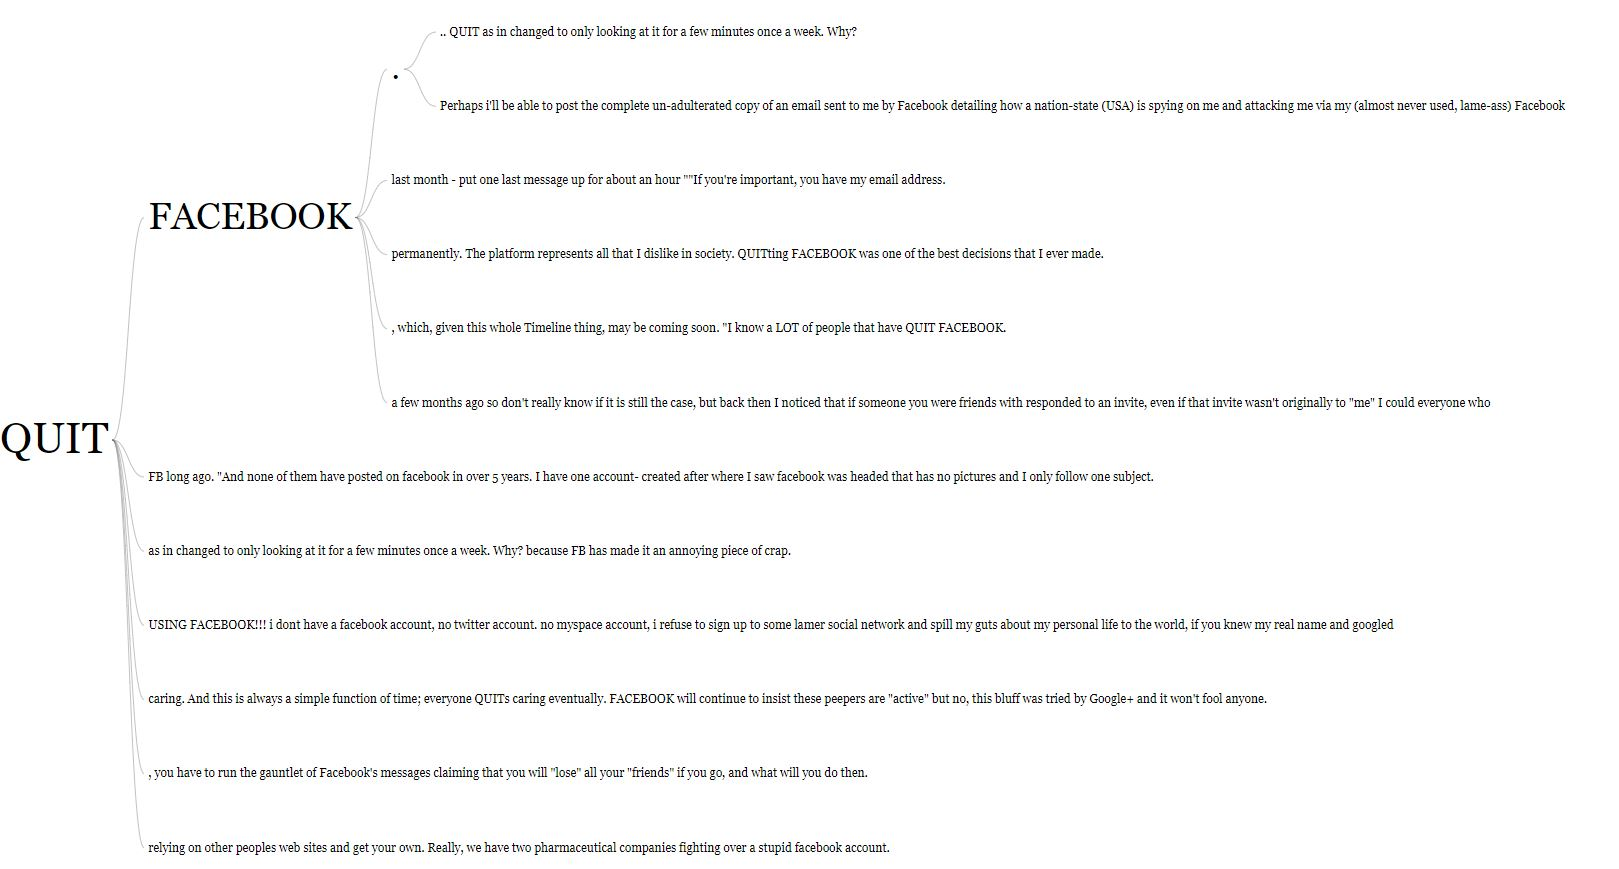
\includegraphics[width=1.0\columnwidth]{figures/WT1.JPG}
  \caption{Partial word tree visualization of  \emph{explicit Non-use} comments of Slashdot}~\label{fig:figure1}
\end{figure*}

\begin{figure*}
  \centering
  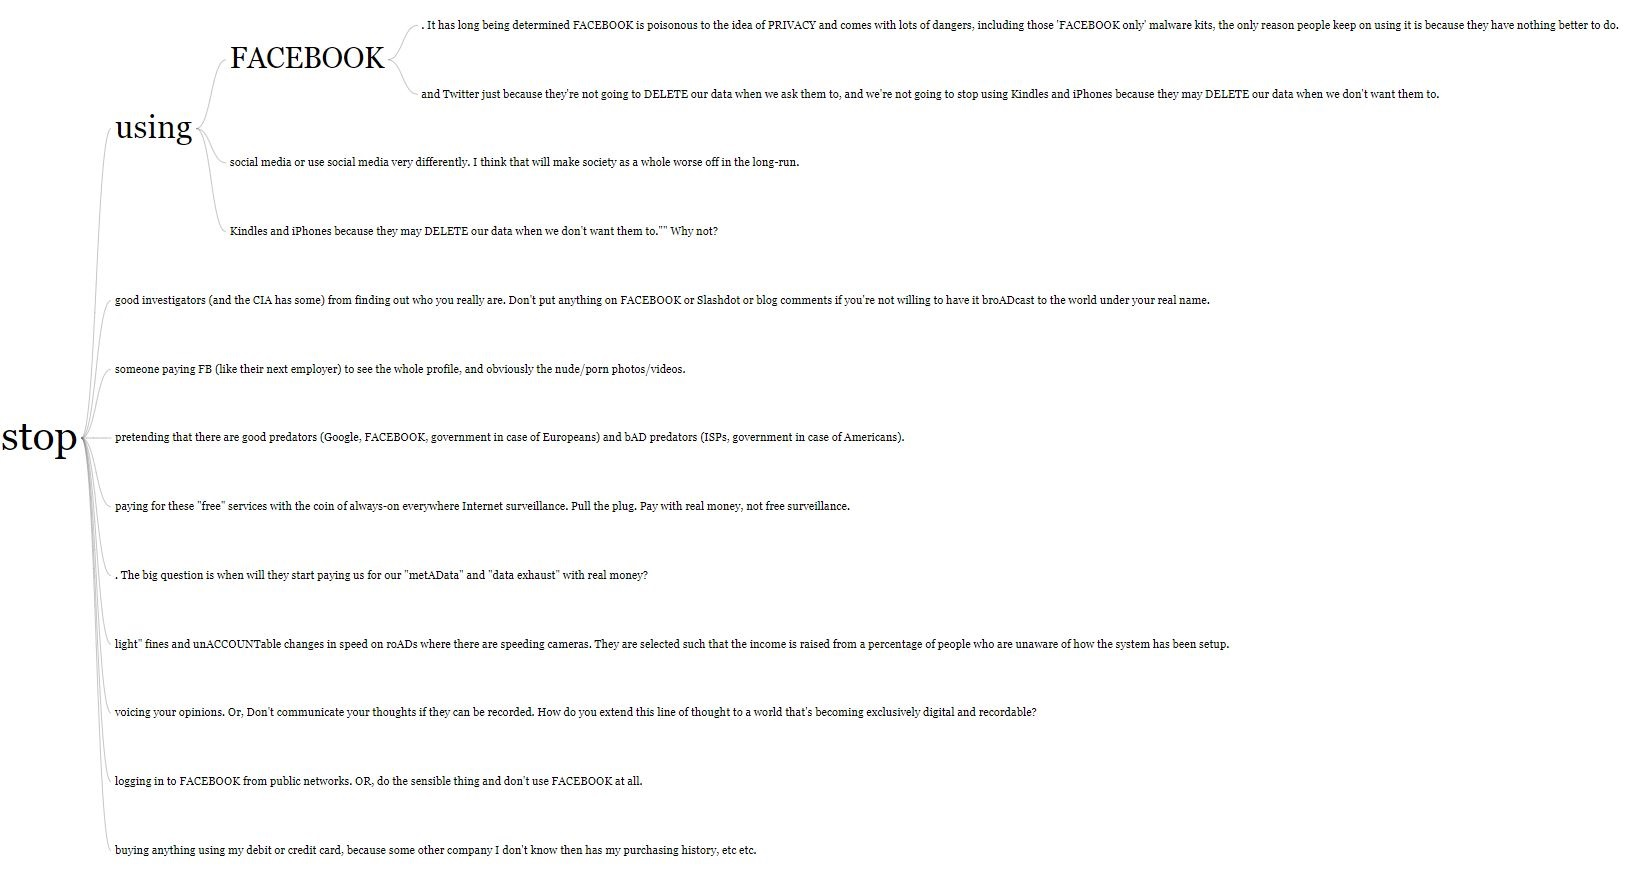
\includegraphics[width=1.0\columnwidth]{figures/WT2.JPG}
  \caption{Partial word tree visualization of  \emph{explicit Non-use} comments of Schneier's blog}~\label{fig:figure2}
\end{figure*}

\end{comment}

\begin{comment}


\begin{table*}[t!]
\centering
\begin{tabular}{|c|c|c|}
\hline
\head{Theme} & \head{\#Comments (Slashdot)} & \head{\#Comments (Schneier's Blog)}  \\
\hline
Politics/Political content     &  5 (0.01\%) & 0 (0\%) \\\hline

Privacy and security concerns  &  138 (44.37\%) & 111 (68.94\%) \\\hline

Uninteresting/unverified content  & 8 (2.57\%) & 12 (7.45\%)\\\hline

Fake accounts/Bots  & 2 (0.64\%) & 8 (4.96\%)\\\hline

User experience   & 118 (37.94\%) & 18 (11.18\%)\\\hline

Switch to other sites/services  & 8 (2.57\%) & 10 (6.21\%)\\\hline



Psychological impact   & 1 (0.32\%) & 3 (1.86\%)\\\hline

Advertisement   & 21 (6.75\%) & 5 (3.1\%)\\\hline

Personal preference  & 42 (13.5\%) & 68 (21.86\%)\\\hline

Other   & 11 (3.53\%) & 14 (8.69\%)\\\hline
\hline
\end{tabular}
\caption{Themes for \emph{explicit Non-use} only comments, number of comments for each dataset.}
    \label{table:coding category non_use_only}
\end{table*}

\end{comment}